% Beamer slides for the ns-3 CAKE paper.
% Build: pdflatex cake-slides ; pdflatex cake-slides
\documentclass[10pt,aspectratio=169]{beamer}
\usetheme{Madrid}
\usecolortheme{seahorse}
\setbeamertemplate{navigation symbols}{}

\usepackage{booktabs}
\usepackage{pgfplots}
\pgfplotsset{compat=1.18}
\usetikzlibrary{positioning,fit,arrows.meta}

\title[ns-3 Model of CAKE]{An ns-3 Model of CAKE}
\subtitle{Design, Validation, and Evaluation of a Comprehensive Queue
Management Discipline}
\author[Wang, Sheng, Zhang]{Haoyu Wang\inst{1} \and Bo Sheng\inst{1} \and Xiaoqian Zhang\inst{2}}
\institute[UMB / UNO]{%
\inst{1}University of Massachusetts Boston \and
\inst{2}University of Nebraska Omaha}
\date{ICNS3 2026}

\begin{document}

% --- 1. Title -----------------------------------------------------------
\begin{frame}
\titlepage
\end{frame}

% --- 2. Bufferbloat -----------------------------------------------------
\begin{frame}{Why this paper: bufferbloat}
\begin{itemize}
  \item Over-buffered network devices inflate latency under load and break
        interactive applications.
  \item In our own measurements: \textbf{a dumb FIFO at 10~Mbit/s sustained
        almost 400~ms of induced latency} under bulk-load.
  \item Active queue management (AQM) addresses this by signalling congestion
        \emph{before} buffers fill.
  \item Today's state-of-the-art AQM in deployment: \alert{CAKE}.
\end{itemize}
\end{frame}

% --- 3. AQM family ------------------------------------------------------
\begin{frame}{From RED to CAKE}
\begin{itemize}
  \item \textbf{RED} (1993): probabilistic drop on average queue.
  \item \textbf{CoDel / PIE} (2012, 2017): delay-controlled drop.
  \item \textbf{FQ-CoDel} (RFC 8290, 2018): per-flow queues + CoDel + DRR.
  \item \textbf{CAKE} (LANMAN 2018): the synthesis, in one qdisc:
    \begin{itemize}
      \item built-in deficit-mode shaper,
      \item per-flow COBALT AQM (CoDel + BLUE),
      \item DiffServ \emph{tins} (priority classes),
      \item TCP ACK filtering,
      \item host-fair triple isolation.
    \end{itemize}
  \item Mainline Linux; behind OpenWrt SQM on millions of home gateways.
\end{itemize}
\end{frame}

% --- 4. The gap ---------------------------------------------------------
\begin{frame}{The gap we close}
\begin{itemize}
  \item ns-3's \texttt{traffic-control} ships RED, CoDel, PIE, FQ-CoDel,
        FQ-COBALT\ldots\ but \alert{not CAKE}.
  \item Researchers who want to compare against CAKE have been approximating
        it with FQ-COBALT, which captures \emph{flow} fairness but \emph{none}
        of CAKE's shaping, DiffServ, ACK filtering, or host fairness.
  \item This paper provides the first ns-3 model of CAKE---and validates it
        against Linux \texttt{sch\_cake}.
\end{itemize}
\end{frame}

% --- 5. Contributions ---------------------------------------------------
\begin{frame}{Contributions}
\begin{enumerate}
  \item First ns-3 model of CAKE, in the \texttt{traffic-control} module,
        reusing the existing COBALT AQM.
  \item A \alert{dependency-clean design} that keeps the model free of
        transport/network header types by injecting header inspection through
        callbacks---a pattern that fits ns-3's module layering.
  \item Validation against Linux \texttt{sch\_cake} (Flent \emph{rrul}) on a
        network-namespace testbed: agreement within $\sim$10\% on throughput
        and $\sim$6\% on latency percentiles, 5--100~Mbit/s.
  \item Released artefacts: model, unit tests, runnable examples, AQM
        comparison campaign, and a reproducible Linux validation harness.
\end{enumerate}
\end{frame}

% --- 6. Architecture ---------------------------------------------------
\begin{frame}{CAKE inside ns-3: architecture}
\resizebox{\textwidth}{!}{%
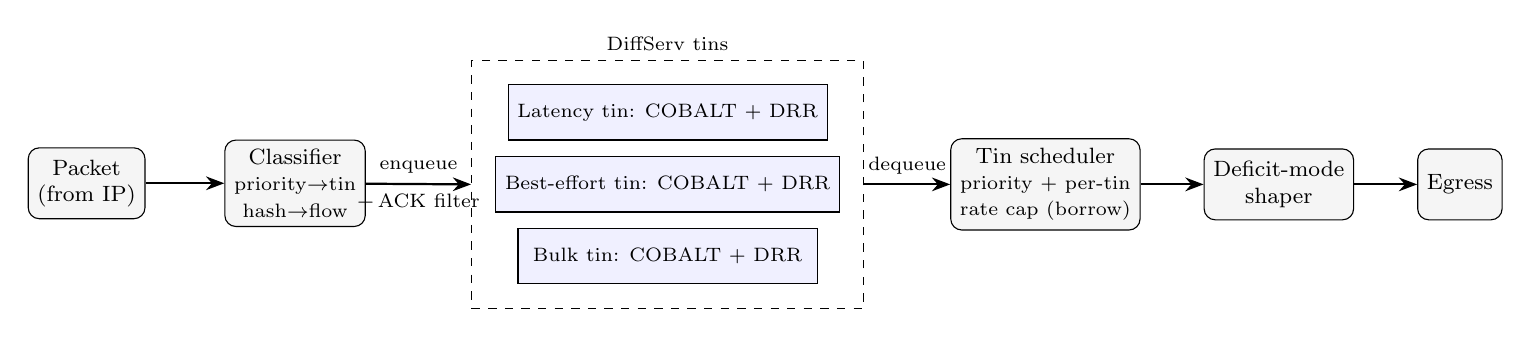
\begin{tikzpicture}[
  >=Stealth,
  box/.style={draw,rounded corners,align=center,minimum height=9mm,font=\footnotesize,fill=gray!8},
  tin/.style={draw,align=center,minimum width=38mm,minimum height=7mm,font=\scriptsize,fill=blue!6}]
\node[box] (in) {Packet\\(from IP)};
\node[box,right=10mm of in] (cls) {Classifier\\{\scriptsize priority$\to$tin}\\{\scriptsize hash$\to$flow}};
\node[tin,right=18mm of cls,yshift=9mm] (t0) {Latency tin: COBALT + DRR};
\node[tin,below=2mm of t0] (t1) {Best-effort tin: COBALT + DRR};
\node[tin,below=2mm of t1] (t2) {Bulk tin: COBALT + DRR};
\node[draw,dashed,inner sep=3mm,fit=(t0)(t1)(t2),label=above:{\scriptsize DiffServ tins}] (tins) {};
\node[box,right=14mm of t1] (sched) {Tin scheduler\\{\scriptsize priority + per-tin}\\{\scriptsize rate cap (borrow)}};
\node[box,right=8mm of sched] (shaper) {Deficit-mode\\shaper};
\node[box,right=8mm of shaper] (out) {Egress};
\draw[->,thick] (in) -- (cls);
\draw[->,thick] (cls) -- node[above,font=\scriptsize]{enqueue} node[below,font=\scriptsize]{+\,ACK filter} (tins.west);
\draw[->,thick] (tins.east) -- node[above,font=\scriptsize]{dequeue} (sched.west);
\draw[->,thick] (sched) -- (shaper);
\draw[->,thick] (shaper) -- (out);
\end{tikzpicture}}
\vspace{1ex}
\small Enqueue: classify $\to$ tin $\to$ flow; ACK-filter marks superseded ACKs.\\
Dequeue: tin scheduler (priority + rate cap, borrowing) $\to$ flow DRR $\to$ shaper.
\end{frame}

% --- 7. Module-boundary pattern (key design contribution) ---------------
\begin{frame}{The hard part: ns-3's module layering}
\begin{block}{Problem}
ACK filtering and host fairness need to inspect TCP and IP headers---but
those types live in the \texttt{internet} module, and
\texttt{traffic-control} \emph{must not} depend on \texttt{internet}.
\end{block}
\begin{block}{Naive ports}
\begin{itemize}
  \item Pull \texttt{traffic-control} into a circular dependency, or
  \item carry knock-off header types inside \texttt{traffic-control}.
\end{itemize}
Both are bad.
\end{block}
\begin{block}{Our pattern: injected callbacks}
\begin{itemize}
  \item \texttt{SetAckIdentifier(\dots)}: ``is this a pure ACK?''
  \item \texttt{SetHostClassifier(\dots)}: ``what are the host keys?''
  \item Concrete implementations supplied by \texttt{internet}:\\
        \texttt{MakeTcpAckIdentifier()}, \texttt{MakeIpv4HostClassifier()}.
\end{itemize}
The core CAKE model stays free of transport/network types.
\end{block}
\end{frame}

% --- 8. Design: shaper + flow isolation ---------------------------------
\begin{frame}{Design highlights (1/2): shaper + flow isolation}
\begin{itemize}
  \item \textbf{Deficit-mode shaper.} Virtual-clock pacing
        ($t_{\text{next}}$ advances by $L/R$ each packet, idle-reset).
        Bandwidth $=0$ disables shaping. Self-wakes via
        \texttt{Simulator::Schedule(\&QueueDisc::Run, this)}.
  \item \textbf{Per-flow isolation.} Reuse the existing
        \texttt{CobaltQueueDisc} as each flow's AQM; set-associative hash
        + new/old-flow DRR (the same machinery as \texttt{FqCobaltQueueDisc}).
  \item In unlimited mode, CAKE collapses to \texttt{FqCobalt}---a useful
        sanity check: our evaluation shows their numbers \emph{exactly}
        match.
\end{itemize}
\end{frame}

% --- 9. Design: tins + ACK filtering + host fairness --------------------
\begin{frame}{Design highlights (2/2): tins, ACK filter, host fairness}
\begin{itemize}
  \item \textbf{DiffServ tins with per-tin rate caps.} Each tin has its own
        virtual-clock shaper at its share of the bandwidth; serve the
        highest-priority \emph{due} tin, else let the least over-budget tin
        \emph{borrow} idle capacity (work-conserving).
  \item \textbf{ACK filtering.} Pluggable identifier; lazy drop at dequeue
        (the ns-3 Queue API removes only from the head, so superseded ACKs
        are flagged and dropped when they reach the head---the saved uplink
        bandwidth is still realised).
  \item \textbf{Host fairness (triple isolation).} Per-flow DRR grant scaled
        by $1/\max(\textit{srcHostLoad}, \textit{dstHostLoad})$, so a host
        with $N$ flows cannot grab $N\times$ its fair host share.
\end{itemize}
\end{frame}

% --- 10. Validation methodology ----------------------------------------
\begin{frame}{Validation methodology}
\begin{itemize}
  \item \textbf{Linux side:} 3-namespace testbed; CAKE on both router egress
        interfaces; \texttt{netem} adds the base RTT at the endpoints;
        Flent's \emph{rrul} test (4 down + 4 up TCP + ping probes).
  \item \textbf{ns-3 side:} an rrul-style scenario in
        \texttt{cake-rrul-validation} that mirrors the topology and traffic.
  \item \textbf{Comparison:} \texttt{cake-validation-compare.py} runs ns-3
        for each Linux reference's parameters and reports per-metric relative
        error with a tolerance gate.
  \item \textbf{Reproducibility:} the testbed script, the Linux references,
        the extract script, and the comparison driver are all checked into
        the module's \texttt{examples/} directory.
\end{itemize}
\end{frame}

% --- 11. Validation: 7-point table -------------------------------------
\begin{frame}{Validation: seven operating points}
\centering
\small
\begin{tabular}{@{}lcccc@{}}
\toprule
Point & Down (Mbit/s) & Up (Mbit/s) & p50 (ms) & p99 (ms)\\
\midrule
1/40    & 0.6 / 0.9   & 0.5 / 0.9   & 48.7 / 61.3   & 71.6 / 90.3\\
5/40    & 4.3 / 4.6   & 4.2 / 4.6   & 43.7 / 44.4   & 49.5 / 51.1\\
10/40   & 8.7 / 9.3   & 8.6 / 9.4   & 41.4 / 42.2   & 43.5 / 45.7\\
20/100  & 16.8 / 18.1 & 16.8 / 18.1 & 100.7 / 101.0 & 101.7 / 103.0\\
50/80   & 44.4 / 44.7 & 42.1 / 45.8 & 80.3 / 80.5   & 80.7 / 81.3\\
100/20  & 93.2 / 93.1 & 93.3 / 93.1 & 20.2 / 20.6   & 20.3 / 23.0\\
100/80  & 85.7 / 89.0 & 85.7 / 88.8 & 80.2 / 80.6   & 80.3 / 82.2\\
\bottomrule
\end{tabular}
\vspace{1ex}
\small ns-3 / Linux. \alert{6 of 7 pass}; the 1~Mbit/s point exposes a
non-rate-adaptive AQM target (a concrete future-work item).
\end{frame}

% --- 12. Validation: scatter + CDFs ------------------------------------
\begin{frame}{Validation: distributional agreement}
\centering
\resizebox{\textwidth}{!}{%
\begin{tikzpicture}
\begin{axis}[width=5cm,height=3.6cm,
  xlabel={Linux (ms)},ylabel={ns-3 (ms)},title={RTT p99},
  xmin=0,ymin=0,xmax=110,ymax=110,
  label style={font=\scriptsize},tick label style={font=\scriptsize},
  title style={font=\small}]
\addplot[no markers,dashed,domain=0:110] {x};
\addplot[only marks,mark=*,mark size=1.5pt] table[x=linux,y=ns3] {validation-rtt.dat};
\end{axis}
\end{tikzpicture}\hspace{2mm}%
\begin{tikzpicture}
\begin{axis}[width=5cm,height=3.6cm,
  xlabel={RTT (ms)},ylabel={CDF},title={CDF @ 50/80},ymin=0,ymax=1,
  label style={font=\scriptsize},tick label style={font=\scriptsize},
  title style={font=\small}]
\addplot[thick,blue] table[x=rtt,y=cdf] {cdf-linux-50-80.dat};
\addplot[thick,red,dashed] table[x=rtt,y=cdf] {cdf-ns3-50-80.dat};
\end{axis}
\end{tikzpicture}\hspace{2mm}%
\begin{tikzpicture}
\begin{axis}[width=5cm,height=3.6cm,
  xlabel={RTT (ms)},title={CDF @ 100/20},ymin=0,ymax=1,yticklabels={},
  label style={font=\scriptsize},tick label style={font=\scriptsize},
  title style={font=\small}]
\addplot[thick,blue] table[x=rtt,y=cdf] {cdf-linux-100-20.dat};
\addplot[thick,red,dashed] table[x=rtt,y=cdf] {cdf-ns3-100-20.dat};
\end{axis}
\end{tikzpicture}}
\vspace{1ex}
\small Most points lie on $y=x$; the 1~Mbit/s outlier sits below it.
The CDFs at 100~Mbit/s reveal a few Linux outliers that the
deterministic simulator does not generate---a fidelity boundary of the
\emph{simulator}, not of CAKE.
\end{frame}

% --- 13. Evaluation: AQM comparison ------------------------------------
\begin{frame}{Evaluation: CAKE among ns-3 AQMs}
\centering
\begin{tikzpicture}
\begin{axis}[width=8cm,height=4.4cm,
  xlabel={Bottleneck rate (Mbit/s)},ylabel={Latency under load (ms)},
  ymode=log,xtick={10,50,100},
  legend pos=north east,legend style={font=\scriptsize,row sep=-2pt},
  label style={font=\footnotesize},tick label style={font=\scriptsize},
  mark size=2pt]
\addplot table[x=rate,y=PfifoFast] {aqm-latency.dat}; \addlegendentry{pfifo\_fast}
\addplot table[x=rate,y=Pie] {aqm-latency.dat}; \addlegendentry{PIE}
\addplot table[x=rate,y=FqCoDel] {aqm-latency.dat}; \addlegendentry{FQ-CoDel}
\addplot table[x=rate,y=Cake] {aqm-latency.dat}; \addlegendentry{CAKE}
\end{axis}
\end{tikzpicture}
\begin{itemize}
  \item Flow-queueing AQMs hold latency near the base RTT at every rate.
  \item Unmanaged FIFO bloats severely (nearly $400$~ms at 10~Mbit/s).
  \item PIE controls delay but \emph{under-delivers throughput} at
        100~Mbit/s (68 vs 97 Mbit/s).
\end{itemize}
\end{frame}

% --- 14. ACK filtering validated ---------------------------------------
\begin{frame}{ACK filtering on asymmetric links (validated)}
\small Flent \emph{rrul} on a 50/1~Mbit/s asymmetric link, 4~down + 4~up.
\vspace{1ex}
\centering
\begin{tabular}{@{}llcc@{}}
\toprule
Config & System & Down (Mbit/s) & RTT p99 (ms)\\
\midrule
ack filter \emph{on}  & ns-3 CAKE & 42.9 & 70.9\\
                      & Linux \texttt{cake} & 42.8 & 70.0\\
ack filter \emph{off} & ns-3 CAKE & 38.5 & 182.3\\
                      & Linux \texttt{cake} & 33.0 & 66.2\\
\bottomrule
\end{tabular}
\vspace{1ex}
\begin{itemize}
  \item With the filter \emph{on}, ns-3 matches Linux within
        \alert{$\sim$1\%} on both throughput and tail latency.
  \item Both systems show the canonical throughput uplift
        (+30\% Linux, +11\% ns-3); $\sim$40k redundant ACKs dropped in 30~s.
  \item Honest divergence: the \emph{off} baseline differs more
        (model vs. Linux scheduling behaviour without the filter).
\end{itemize}
\end{frame}

% --- 15. Limitations & future work -------------------------------------
\begin{frame}{Limitations \& future work}
\begin{itemize}
  \item \textbf{Low-rate over-drop.} Fixed CoDel target; Linux scales the
        target with the configured rate (\texttt{cake\_set\_rate}). Closing
        this gap fixes the 1~Mbit/s validation point.
  \item \textbf{Lazy ACK removal.} The ns-3 \texttt{Queue} API removes only
        from the head; an extended interface would allow Linux-style
        in-place splice.
  \item \textbf{IPv4 only} in the provided header-inspection callbacks.
  \item \textbf{Simulator-level jitter.} The deterministic simulator does
        not reproduce kernel-scheduling / NIC-interrupt outliers visible in
        Linux's right tail at 100~Mbit/s.
\end{itemize}
\end{frame}

% --- 16. Conclusion ----------------------------------------------------
\begin{frame}{Conclusion}
\begin{itemize}
  \item First ns-3 model of CAKE---flow isolation, shaper, DiffServ tins
        with per-tin rate caps, ACK filtering, host-fair triple isolation.
  \item A small \alert{module-boundary pattern} (injected header-inspection
        callbacks) keeps the model dependency-clean and unblocks ports of
        other header-aware mechanisms.
  \item Validated against Linux \texttt{sch\_cake} over Flent \emph{rrul}:
        $\sim$10\% throughput, $\sim$6\% tail-latency agreement, 5--100~Mbit/s.
  \item Model, tests, examples, and the validation harness are released
        with the paper for inclusion in ns-3.
\end{itemize}
\begin{center}
\Large\alert{Thanks --- questions?}
\end{center}
\end{frame}

\end{document}
